\chapter{System Overview}
  Since my goal was to quickly influence the lives of real people
  and better understand the methods of communication likely to be used by
  modern people in the near future, I chose to design
  a mobile application, now called InMind.
  The application icon is shown in figure \ref{fig:application_icon}

  \begin{figure}
  \centering
  
\includegraphics[width=0.3\textwidth]{inmind_logo2.png}
  \caption{InMind is an Android Application,
  which lives on users' personal devices,
  so that it is available during the day.}
  \label{fig:application_icon}
  \end{figure}

  InMind would enable a kind of slow,
  targeted communication that had been useful to bereaved individuals in forums,
  but connect individuals with people that they choose.

  \section{Interaction Design}
  Broadly, the goal of the application was to create support groups and 
  enable users within that group to create spaces
  with themed topics, that had a status of some nature.
  This status could represent the user's well being, the well being of someone else
  that the user cares about, the progress of a project, the energy level of a group,
  the level of anxiety the user is suffering from, etc.
  Since mobile applications are always accessible,
  these themed spaces could be updated at any point
  during the day when the status of that topic changes.
  At any point during the day,
  the user can choose to open the app and create or update a topic.
  Figure \ref{fig:user_interaction} shows the user activities
  that are likely, along with the application view screens that are involved.
 
  \begin{figure}
  \centering
  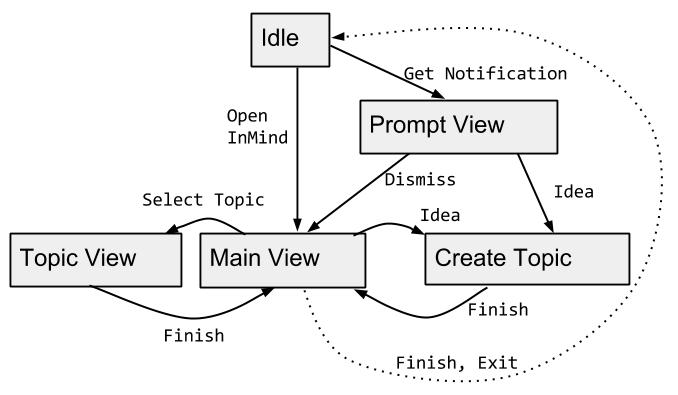
\includegraphics[width=0.7\textwidth]{user_interaction.jpg}
  \caption{Flowchart of likely user interactions on InMind.}
  \label{fig:user_interaction}
  \end{figure}

  Finally, since individuals have shown to be sensitive
  to which particular people they share
  sensitive topics with \cite{patil05},
  the users can choose when they begin the topic
  which of their people they want to share with.

  To summarize, once shared, the topics would be defined by several characteristics:

  \begin{enumerate}
  \item \textbf{Title} - Answers the question of \textbf{What}. The user can choose what to call the topic.
  \item \textbf{Share With} - Answers the question of \textbf{Who}.The topic is like a static chatroom,
    since the people who are listening in are always the same.
  \item \textbf{Status} - Answers the question of \textbf{How}. The "status icon" of the topic sets the mood
    of the topic. Unlike for chatrooms,
    this status allows the space to reflect the state
    of the user who started the topic.
  \end{enumerate}

  Within those spaces, we wanted to encourage communication.
  Here, although I was inspired by the nature of online forums,
  where many people reach out for support,
  our goal was more influenced by the nature of mobile communications.
  On a mobile device, users expect to use abbreviated conversation.
  Although the thoughts may be complex, the messages composed on a mobile device
  tend to be very short.

    \subsection{User Model}
      It is interesting to note that the user interactions within a group
      are likely asymmetric on several fronts.
      On each individual topic, there is a significant difference between the owner
      and the users that were invited to share the topic.
      The topic life cycle and available interactions for the owner
      and those people the owner shares the topic with
      is shown in figure \ref{fig:topic_lifecycle}.

        \begin{figure}
        \centering
        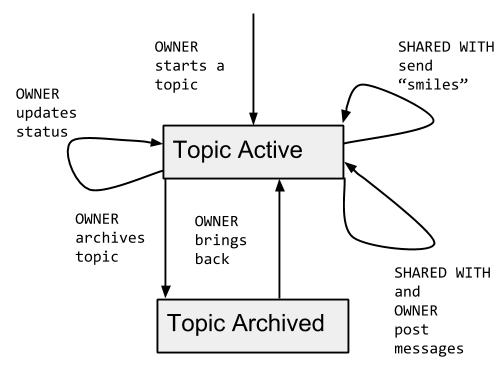
\includegraphics[width=0.6\textwidth]{topic_lifecycle.jpg}
        \caption{Topic lifecycle and possible interactions.
        The Owner creates the topic, and is in control of its status,
        as well as its archive state.
        The people the topic is Shared With can comment and send smiles.}
        \label{fig:topic_lifecycle}
        \end{figure}

      The owner is able to control the state of the topic,
      and thus has the power to control the theme of the conversation.
      This becomes an outlet of expression for the owner,
      as he can shape the icon to represent the status of the topic,
      and thus discuss the topic knowing that the group understands the status as well.

      Another asymmetry is that it is very likely that most groups will
      have asymmetric participation.
      Some members will be eager to begin topics, initiate discussions,
      and others less so.
      This is anticipated in the design,
      as people have differing needs for communication,
      but the application will encourage ownership of at least a topic or two,
      otherwise the "Mine" filter will remain very empty.

  \section{Android Application}

    \subsection{Platform Choice}
    The application was written for Android, targeting API 18,
    but supports down to API 13.

    I chose to develop in Android partially because the Affective Computing Group
    has a recent tradition for doing so.
    This is for reasons related variously to the freedoms that Android developers have,
    and the availability of third party software toolboxes for Android.
    However, my primary reason for choosing Google Android over Apple iOS is
    the prevalence of Android devices.
    Android has been dominating the mobile market since 2012,
    and if InMind were to be released to the public,
    an Android application is more likely to reach out to a broader audience.

    The InMind application supports API 13 through 18, 
    corresponding, respectively, to Android 3.2 Honeycomb and 4.3 Jellybean.

    Android 4.3, Jellybean, was released the year ago, but is by far
    the most prevalent in the MIT target population due to the devices
    that supported it sold over the course of the year.
    During development, Android 4.4, KitKat is being pushed out to devices,
    but yet isn't available to a significant degree.

    At the opposite end, API 13, was released with Android 3.2 HoneyComb
    in 2011, 3 years prior to this date of writing.
    Mobile devices have a life span of about two years,
    and thus it is unlikely for Android users to be
    running versions of Android older than API 13.

    \subsection{Hardware}
    InMind has to integrate into a user's existing communication methods,
    as that is the environment actually encountered in the lives of people.
    Thus, emulating more typical applications,
    InMind is designed to be installed onto the user's existing mobile device.

    As previously suggested by the range of compatible Android versions,
    InMind is designed to be run on an assortment of devices.
    
    In addition to version issues, Android devices vary significantly in form factor.
    The two most popular are cell phone-like devices, which have roughly a 4" screen,
    and small tablets, which have roughly a 7" screen.

    I developed primarily on two devices, a Samsung S4, with a 4" screen,
    and a 2012 Nexus 7, with a 7" screen.
    Design objectives for all layouts was to be attractive on the cell-phone-sized screens,
    and reasonably functional on larger tablet screens.

    \subsection{Application Structure}
    The interactive part of the application is best described by a description of the views
    and the actions available to the user on them.
      \subsubsection{Main View}
      The main view shows the topics that the user has access to.
      See figure \ref{fig:home_screen} for a series of screenshots of the home page design.

    \begin{figure}
      \caption{\textbf{Main View} --
          (a) The main view has a sliding window of topics.
          Topic icons are prominently displayed,
          as are the topic titles and owners.
          Topics that have updates are highlighted with a yellow glow.
          (b) Since there can many topics shared withi the group,
          the main view has filters that can show a subset of the topics.
          (c) Users can make their own collections to sort topics
          the way they want to.}
      \centering
      \begin{subfigure}[b]{0.3\textwidth}
        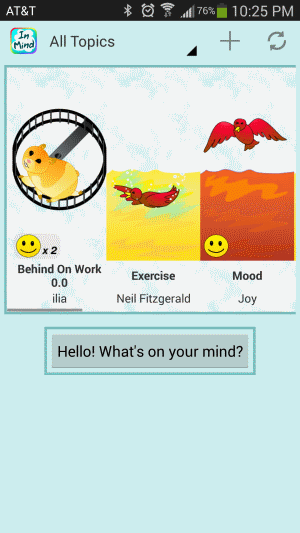
\includegraphics[width=\textwidth]{home_view.png}
         \caption{Main Home view}
      \end{subfigure}
      \begin{subfigure}[b]{0.3\textwidth}
        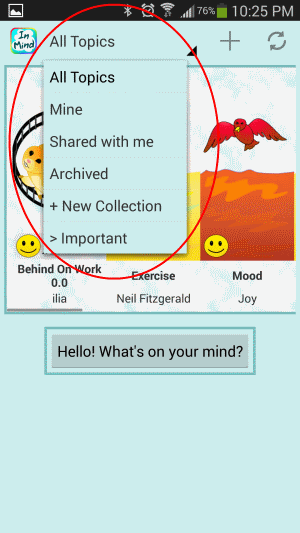
\includegraphics[width=\textwidth]{home_nav.png}
        \caption{Filters}
      \end{subfigure}
      \begin{subfigure}[b]{0.3\textwidth}
        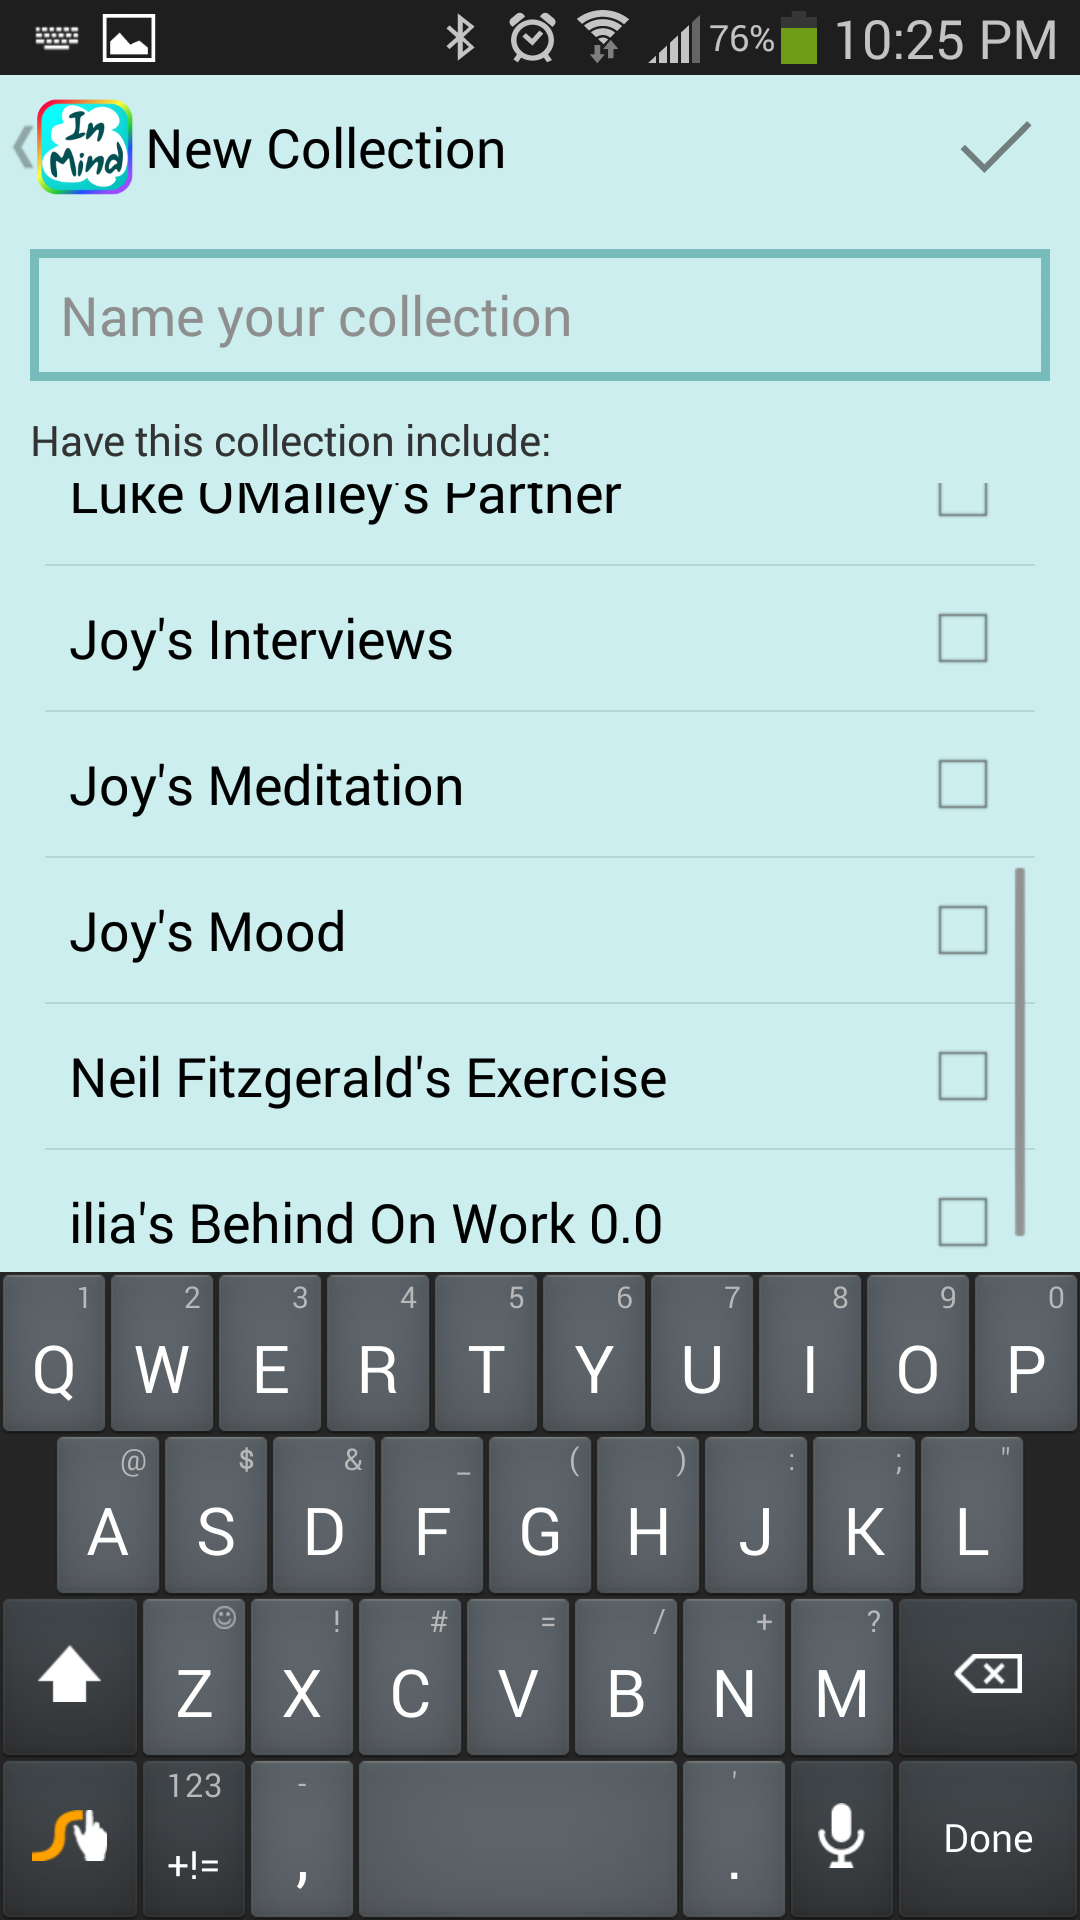
\includegraphics[width=\textwidth]{new_collection.png}
        \caption{New Collection}
      \end{subfigure}
      \label{fig:home_screen}
    \end{figure}

      Since the iconography of the topics is very important,
      the main page gathers the icons of the topics in a scrolling view.
      Each topic is labeled with its title and owner.
      Whenever a topic is updated, whether with a message from someone,
      or with a status change, everyone who can see the topic will see the topic
      lit up with a yellow glow, indicating that there is something to see under that topic.

      As the number of topics increases,
      it becomes increasingly important to have a way to organize the topics.
      I chose to implement this in the form of filters.
      The filters are available in a dropdown menu in the action bar at the top of the screen.
      (The second screenshot in figure \ref{fig:home_screen})
      There are three default filters that always filter for topics that meet certain criteria.
      The first two are "Mine" and "Shared with Me"
      which filter for, respectively, topics the user has created and those he did not.
      The last is "Archived" which shows only the archived topics.
      Archived topics do not appear in any other filtered view.

      Finally, the user can create their own filters.
      The filter creation page is shown in the third screenshot in figure \ref{fig:home_screen}.
      The freedom to create their own filters allows users to organize
      their topics however they like.
      Some ideas include bringing out topics that are particularly important,
      particularly serious or un-serious, created by specific people,
      or even filtering by higher level themes.

      \subsubsection{Creation View}
      When a user want to initiate the topic,
      they can click the add button on the action bar at the top of the home page.
      This opens up the creation view, which is shown in figure \ref{fig:topic_create}.
      On this page, the user titles the topic,
      chooses an icon, and chooses who to share the topic with.

    \begin{figure}
      \caption{\textbf{Creation View} --
          (a) Topic creation involves naming the topic,
          choosing the icon type,
          and choosing who to share the topic with.
          (b) A dropdown menu allows users to choose which icon
          represents the topic.}
      \centering
      \begin{subfigure}[b]{0.4\textwidth}
        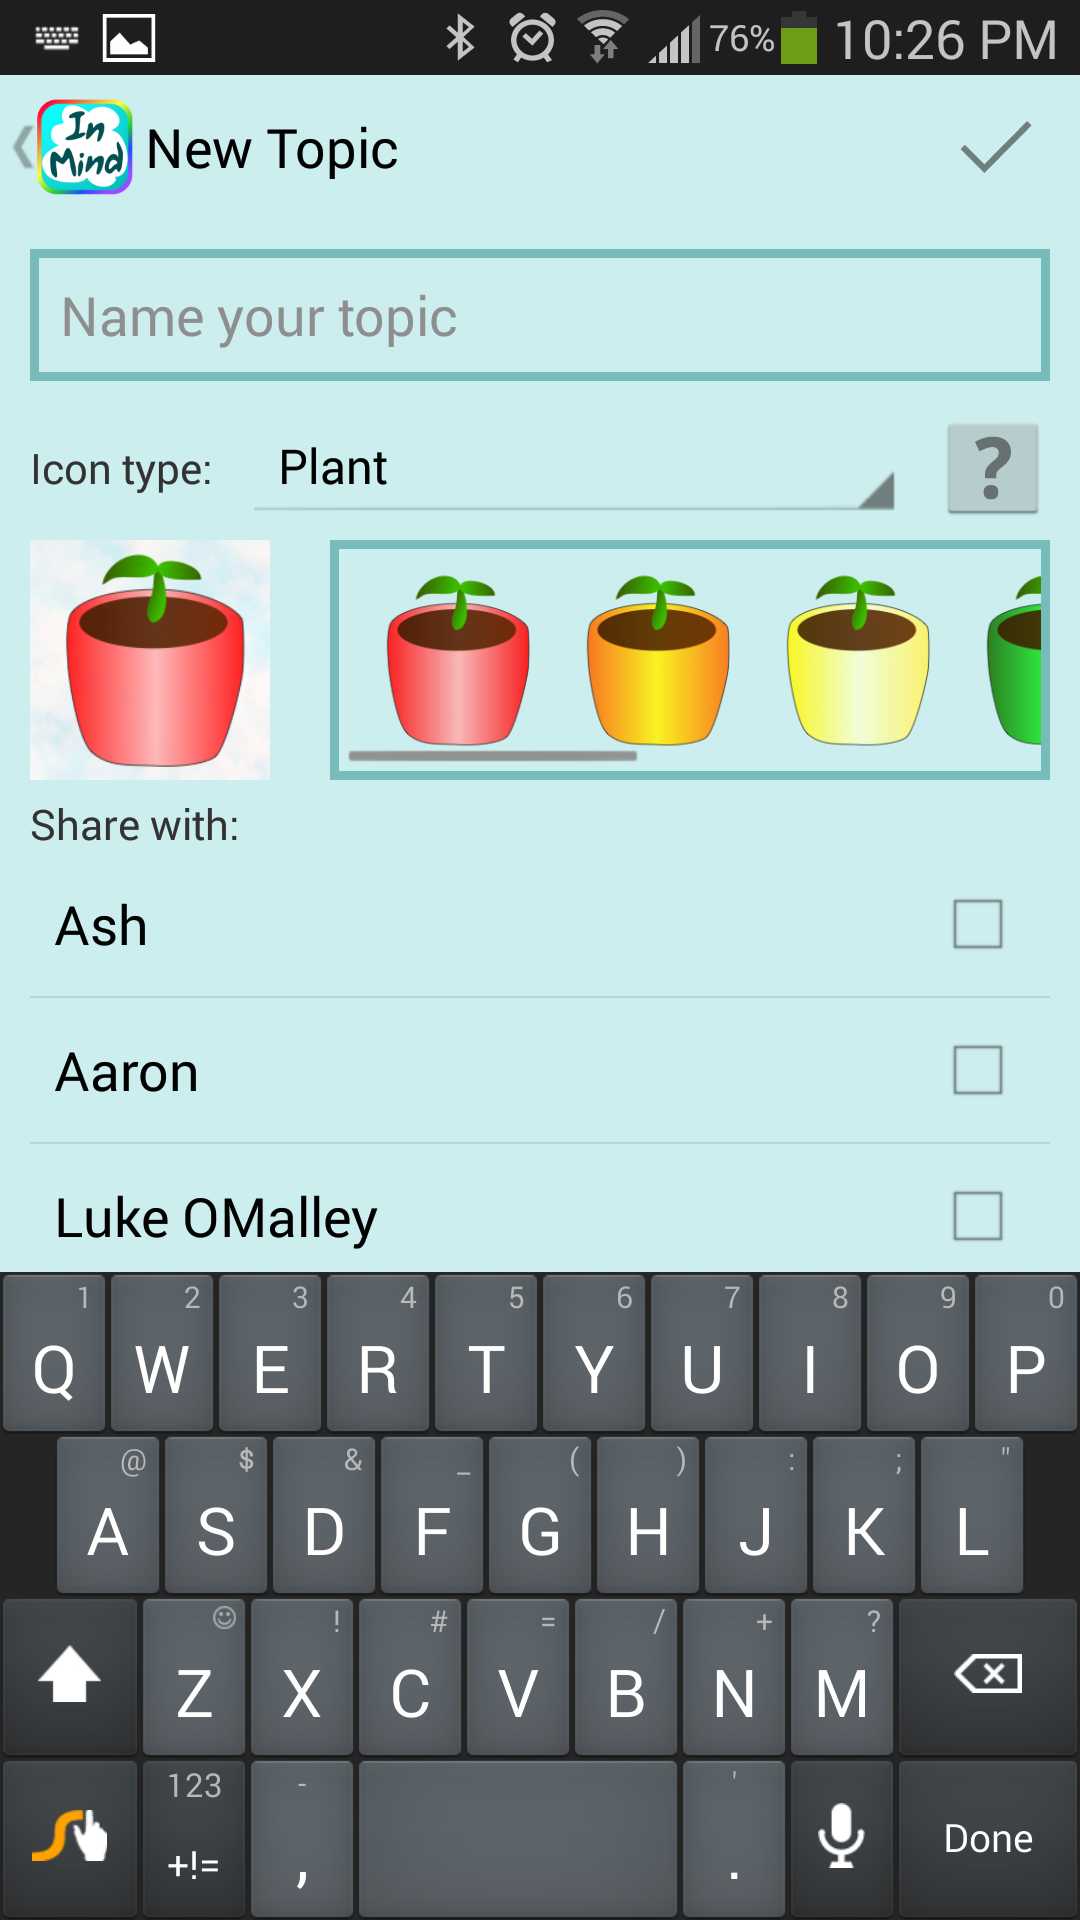
\includegraphics[width=\textwidth]{topic_create.png}
         \caption{Create Topic}
      \end{subfigure}
      \begin{subfigure}[b]{0.4\textwidth}
        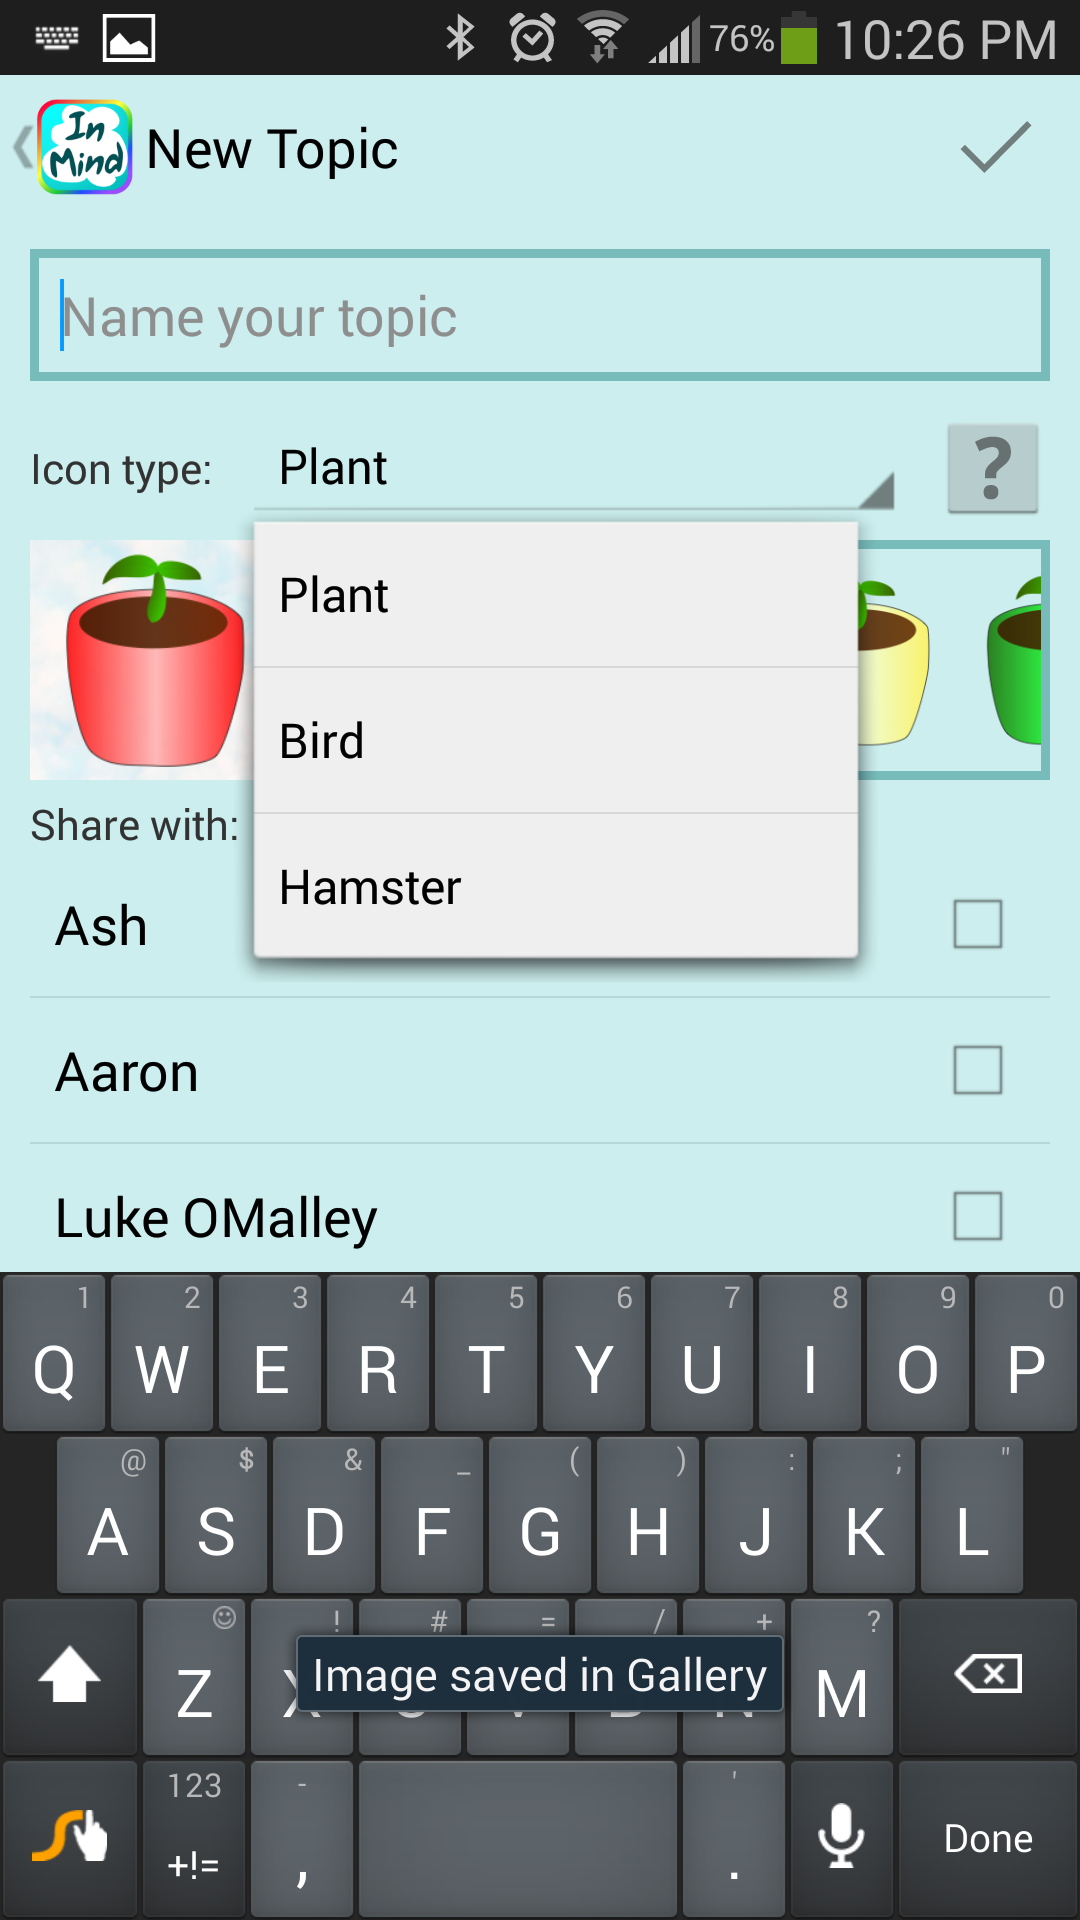
\includegraphics[width=\textwidth]{topic_create_choose.png}
        \caption{Choose Icon Type}
      \end{subfigure}
      \label{fig:topic_create}
    \end{figure}

      The choice of the icon is very important in setting the theme of the topic.
      First, let me explain the structure of InMind status icons.
      The icons are of three kinds: plants, birds, and hampsters.
      All three icons are of a similar structure, and have two parts.
      \begin{enumerate}
      \item A background color, to make the icon distinct from others like it.
      \item A "character" icon, whose status changes between 5 to 8 different levels.
      \end{enumerate}

      As previously mentioned, the icon is very important in setting
      the theme for the topic, since its state represents the status of the topic
      in reality.
      The design of the icons is very important in influencing how
      the users interact with the topics. 
      There are three kinds of icons, and they represent three types of statuses.
      \begin{enumerate}
      \item \textbf{Plants} grow in a colored pot. They are a good general purpose icon as they are neutral,
      not personable, and a familiar icon in many other settings,
      since they are associated with positive feelings of growth.
      \item \textbf{Birds} are positioned relative to a colored water level.
      They indicate affective wellness or degree of success in the face of difficulty.
      \item \textbf{Hamsters} run on a colored exercise wheel.
      Their speed can represent arousal,
      or associated energy levels for the topic.
      \end{enumerate}
      The progression of icons is completely detailed in the appendix,
      and a few sample icons are shown in figure \ref{fig:icon_types}.

    \begin{figure}
      \caption{\textbf{Icon Types}
        (a) Plants represent progress.
        (b) Birds represent wellness or general status.
        (c) Hamsters represent activity or arousal.
      }
      \centering
      \begin{subfigure}[b]{0.3\textwidth}
        
\includegraphics[width=.7\textwidth]{ic_plant2.png}
         \caption{Plant}
      \end{subfigure}
      \begin{subfigure}[b]{0.3\textwidth}
        
\includegraphics[width=.7\textwidth]{ic_bird3.png}
        \caption{Bird}
      \end{subfigure}
      \begin{subfigure}[b]{0.3\textwidth}
        
\includegraphics[width=.7\textwidth]{ic_hamster2.png}
        \caption{Hamster}
      \end{subfigure}
      \label{fig:icon_types}
    \end{figure}

      The symbology was unclear to early beta testers,
      suggesting that choosing an appropriate icon for a topic can be difficult.
      The topic creation page helps by providing
      a short blurb to describe how to use each icon type.

      \subsubsection{Topic View}
      From the home page,
      the user can select a topic to jump to that topic's page.
      Screenshots of the topic page can be seen in figure \ref{fig:topic_view}.

    \begin{figure}
      \caption{\textbf{Topic View} --
          Topic views show the topic's current status icon,
          controls available to the user,
          and messages that have been left under that topic.
          Messages have been blurred, and controls are circled in red.
          (a) If you own a topic, you can adjust its status.
          (b) On someone else's topic, you can leave a smile.
          (c) You can see only your own archived topics,
          and you can bring them back from the archive
          and read the messages attached to it.}
      \centering
      \begin{subfigure}[b]{0.3\textwidth}
        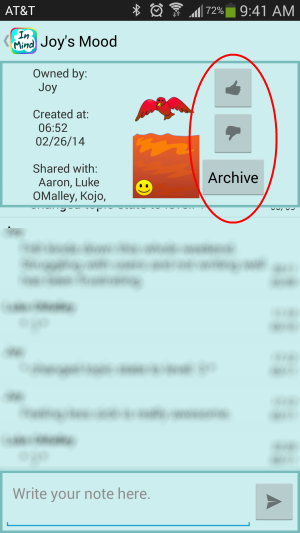
\includegraphics[width=\textwidth]{topic_view_mine.png}
         \caption{My Topic}
      \end{subfigure}
      \begin{subfigure}[b]{0.3\textwidth}
        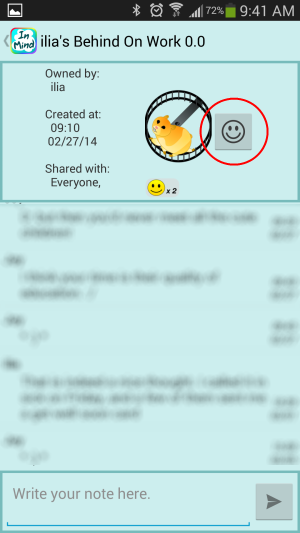
\includegraphics[width=\textwidth]{topic_view_other.png}
        \caption{Someone Else's Topic}
      \end{subfigure}
      \begin{subfigure}[b]{0.3\textwidth}
        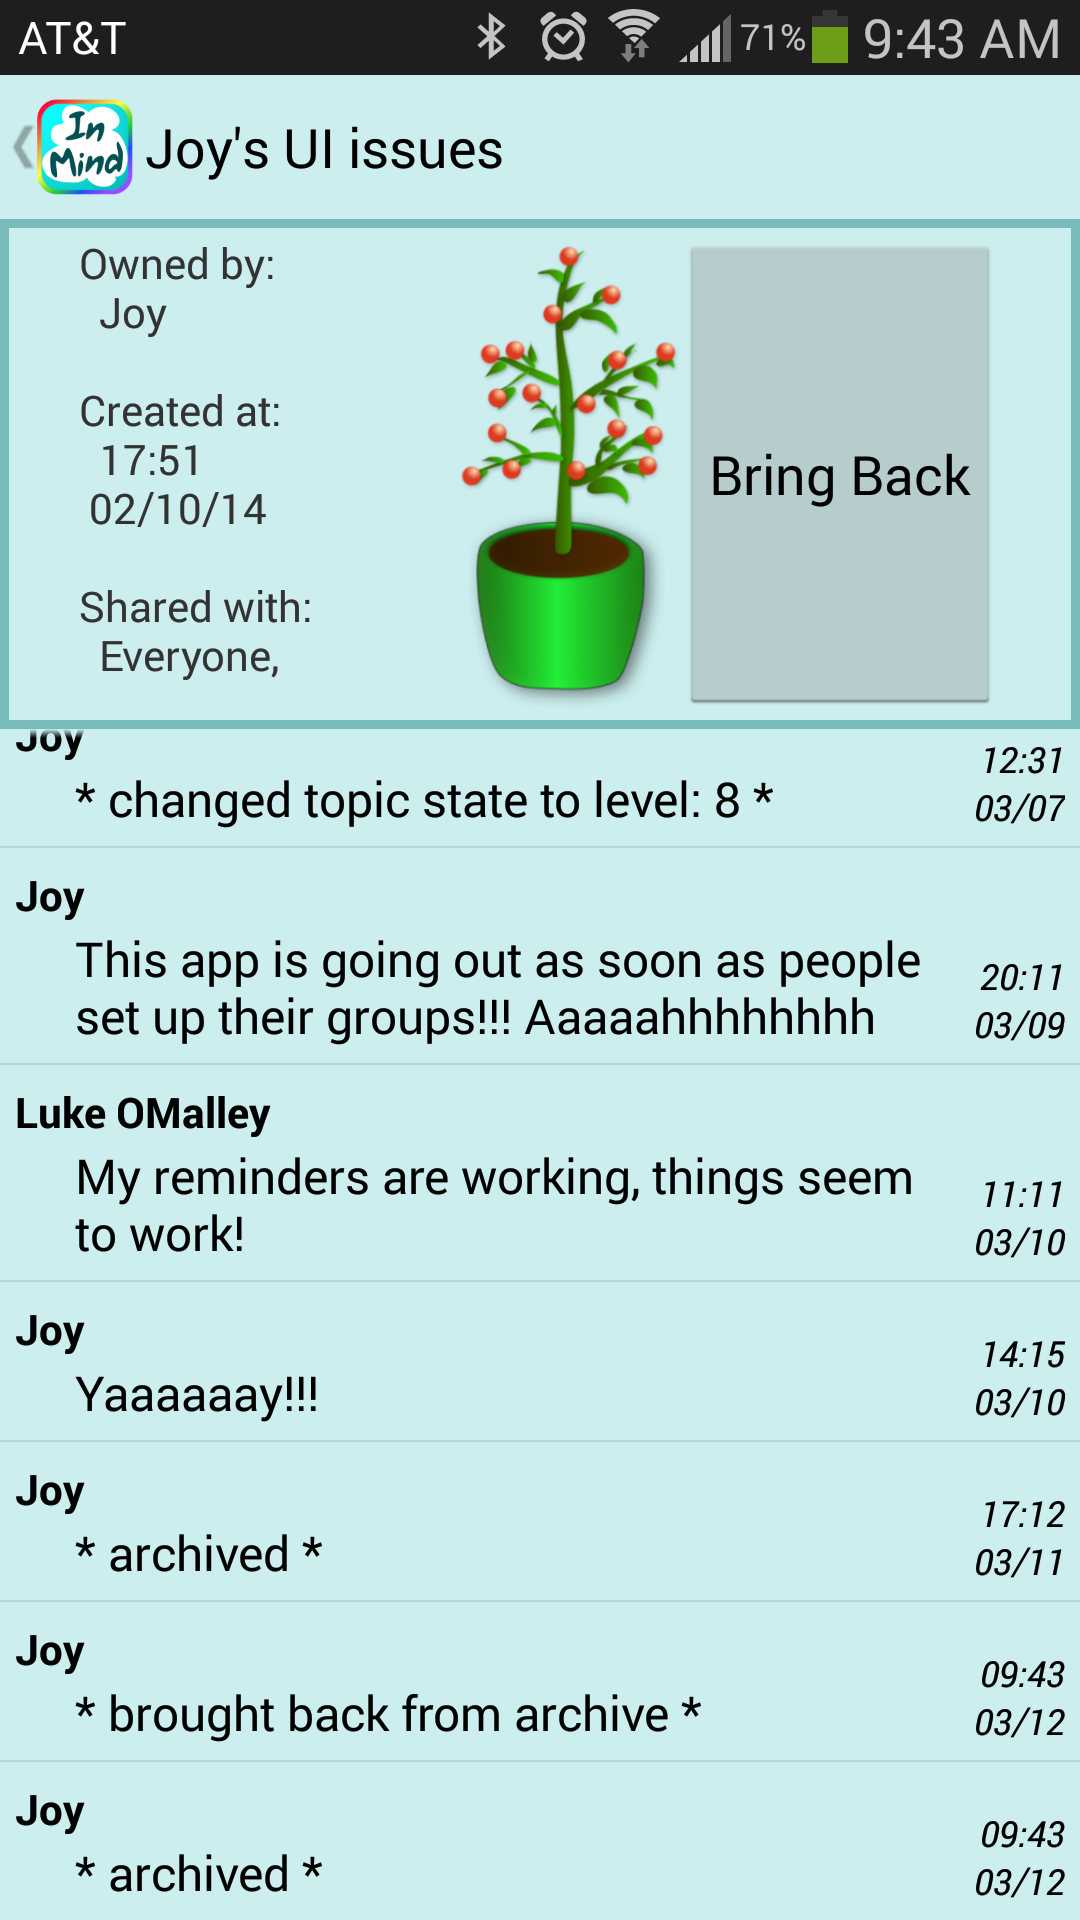
\includegraphics[width=\textwidth]{topic_view_archived.png}
        \caption{Archived Topic}
      \end{subfigure}
      \label{fig:topic_view}
    \end{figure}

      The topic page is primarily modeled after a chatroom,
      or more common on the mobile device platform,
      a text message log.
      The previous messages in that topic are displayed on the main view,
      in reverse chronological order, similar to most chatroom and text message application.

      A button near the top toggles the appearance of a panel that shows data and controls
      related to the topic.
      The data panel has a text section with the topic creation date and who the topic is shared with.
      The current icon for the topic is shown, as expected, as are 3 buttons for controls.

      With the first two buttons,
      the owner of a topic can increase or decrease the state of the icon.
      These changes are logged in the message logs,
      so that people with whom the topic has been shared with
      can also track the status of the topic.

      The last button allows the owner to archive a plant,
      effectively freezing the plant and constraining it to the archive view.
      Archived plants also have a similar view,
      but the status change and messaging capabiliies are disabled.
      Archived plants provide a record of interactions,
      but cannot be interacted with further unless they are brought out of the archive.

      \subsubsection{Prompts and Notifications}
      InMind has a daily notification system.
      InMind chooses a random hour between 9:00 A.M. and 3:00 P.M.,
      and another hour between 4:00 P.M. and 9:00 P.M. to show a notification.

      The notification first appears as a small icon in the status bar,
      in the upper left hand corner of
      the mobile screen, which is visible no matter what the user is doing on their phone.
      The notification appears on the Android notification drawer,
      which the user sees when they drag the notification drawer down.
      On selection,
      the notification sends the user to InMind,
      and shows a dialog with the prompt of the day.
      The prompt in the dialog changes every day,
      and is chosen random from a bank of 180 prompts,
      either a thoughtful quote or a question,
      that is designed to help encourage creative topic creation.
      See the screen shots in figure \ref{fig:notification} to see the progression
      from notification to the application.

    \begin{figure}
      \caption{\textbf{Notification System} --
        InMind's daily notifications remind the user to check the application
        for updates from other users and new prompts.
        (a) The notification first appears as a small icon on the
        Android status bar.
        Also displayed is the InMind application icon on the Android launcher.
        (b) Opening the Android notification drawer shows the InMind notification.
        (c) Clicking it navigates to the application, where a prompt is displayed.
        The prompt dialog box displays a quote or a question,
        and allows the user to just to a topic creation if desired.}
      \centering
      \begin{subfigure}[b]{0.3\textwidth}
        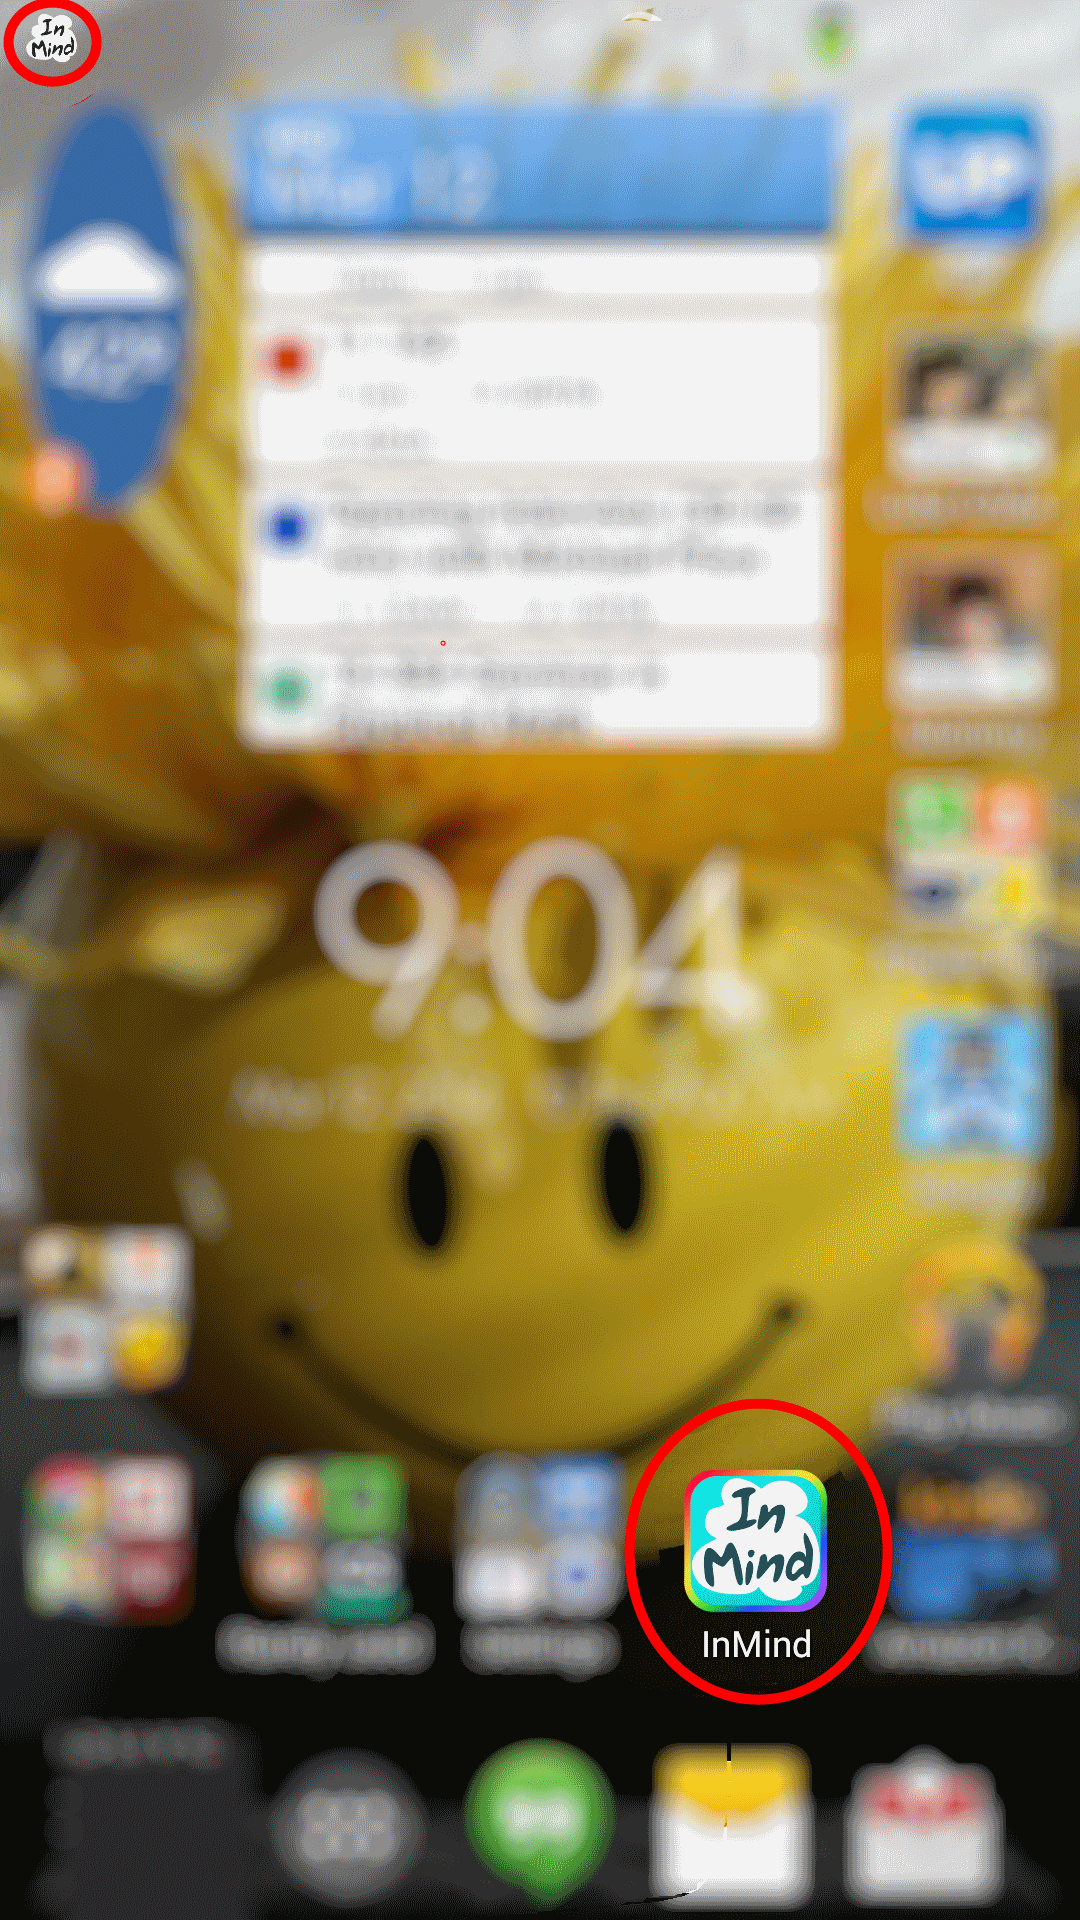
\includegraphics[width=\textwidth]{android_launcher.png}
         \caption{Icons}
      \end{subfigure}
      \begin{subfigure}[b]{0.3\textwidth}
        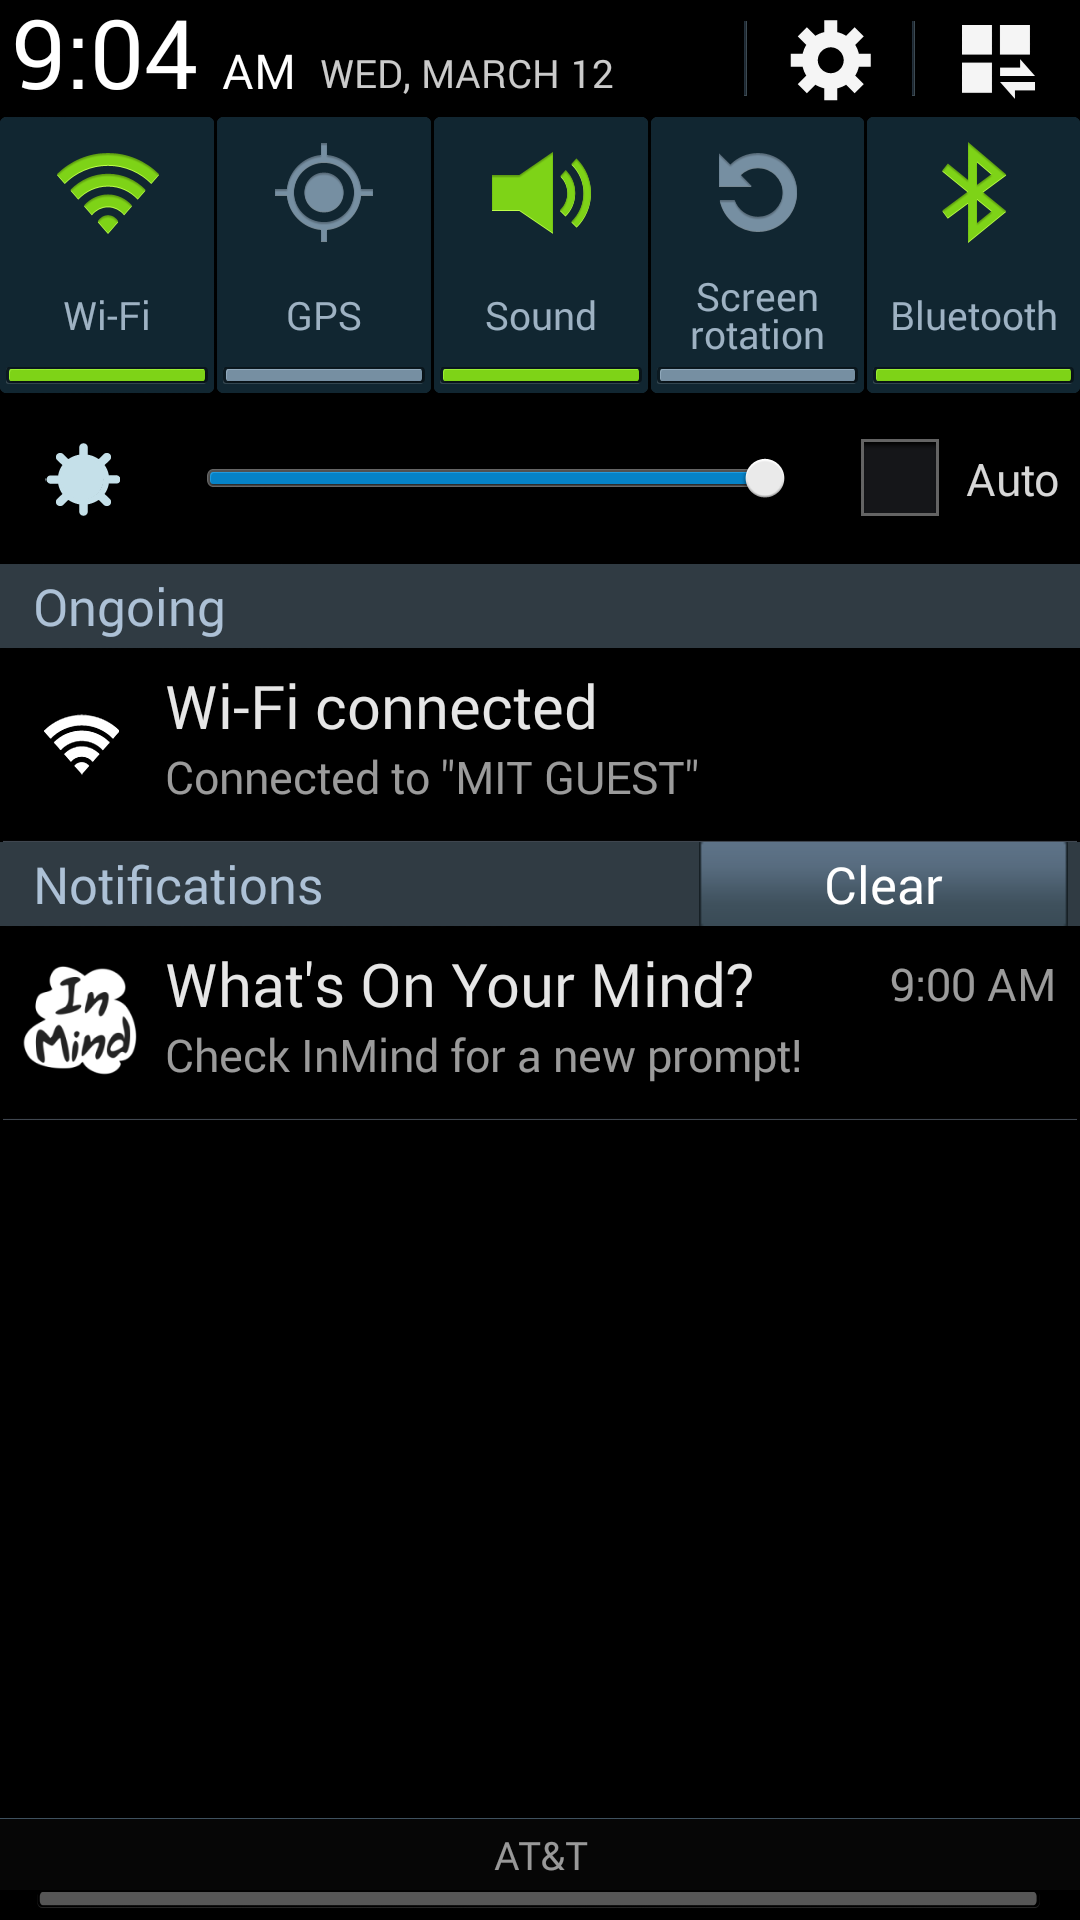
\includegraphics[width=\textwidth]{notification.png}
        \caption{Notification Drawer}
      \end{subfigure}
      \begin{subfigure}[b]{0.3\textwidth}
        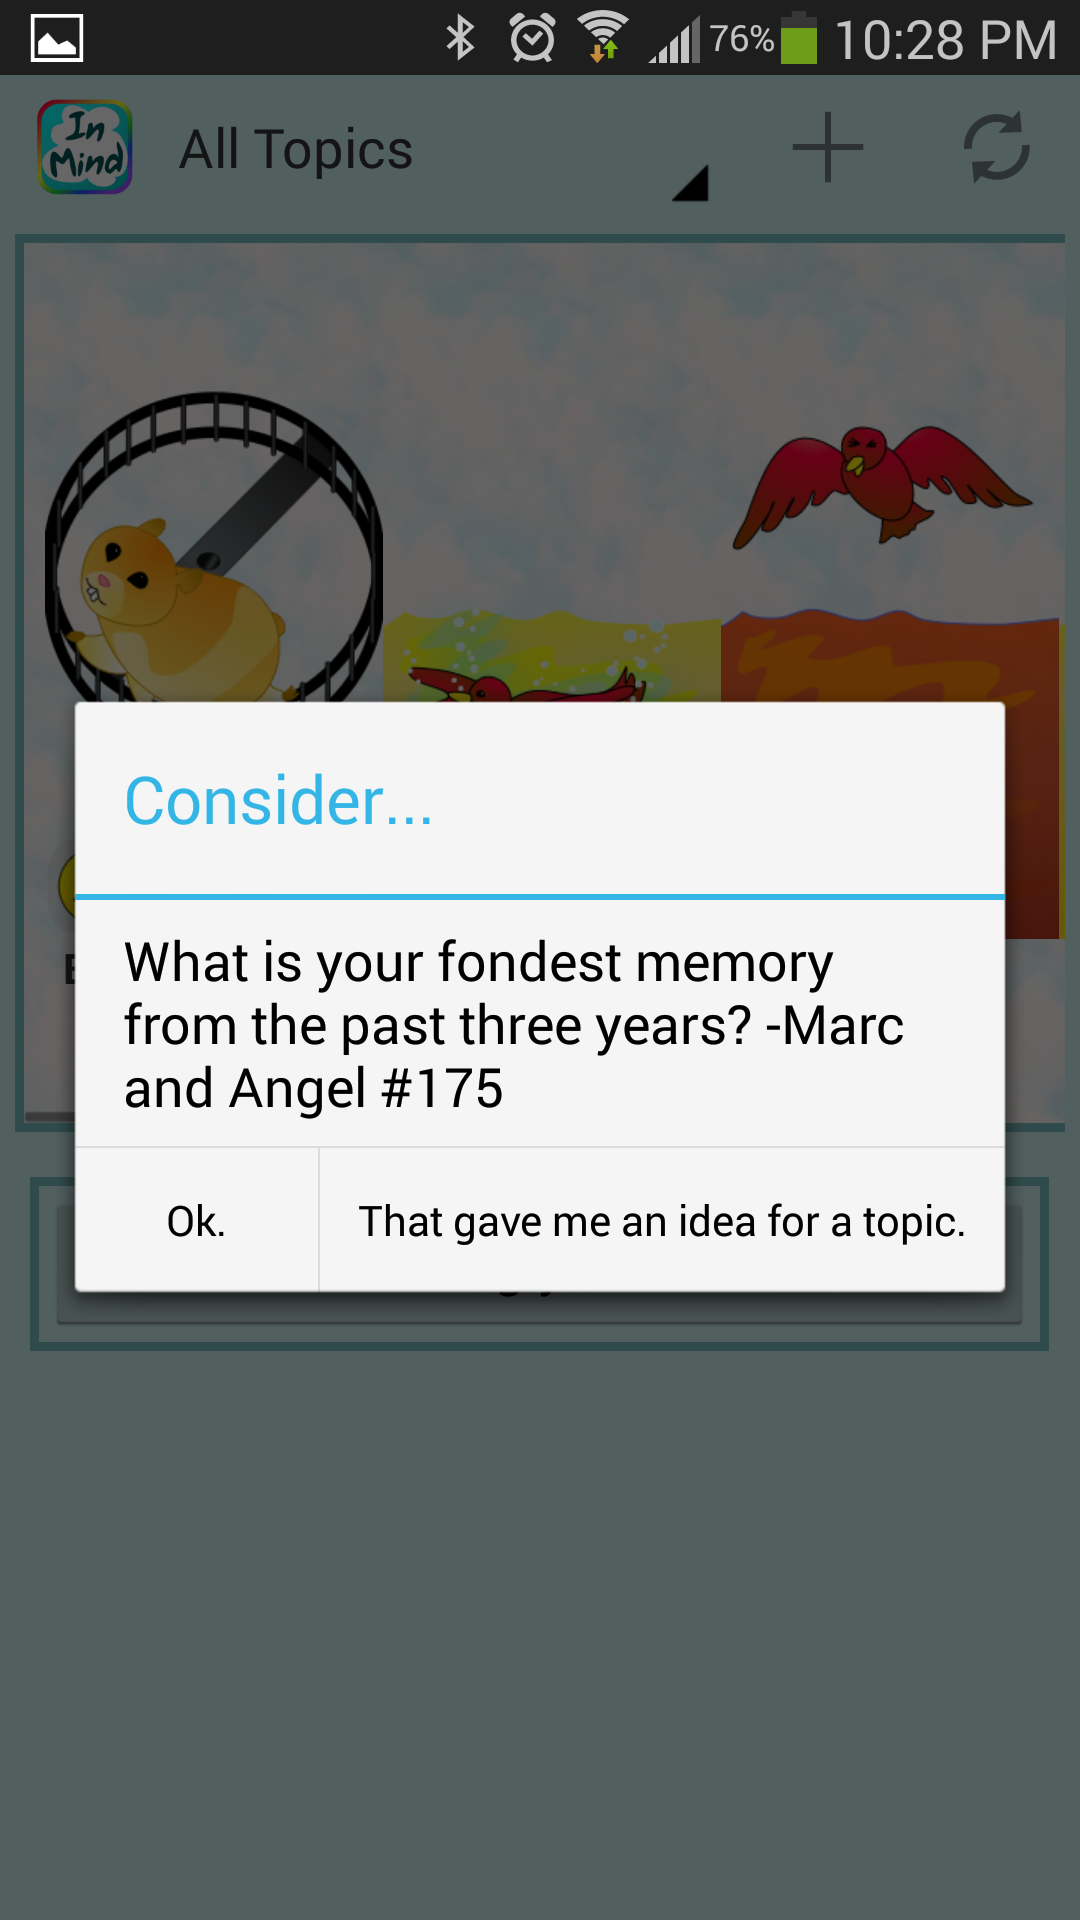
\includegraphics[width=\textwidth]{prompt_dialog.png}
        \caption{Prompt Dialog}
      \end{subfigure}
      \label{fig:notification}
    \end{figure}

      To see the prompt again, the user can use a small button
      below the scrolling view of topics that displays the topics
      that match the filter.

    \subsection{Security}
      Due to the sensitive nature of the application,
      many measures have been taken for security purposes.
      Although most security concerns are handled by the server,
      two were necessary on the application end.

      First, since the topics and their corresponding messages may be private in nature,
      possibly even more private than the other material storied on the device,
      there is an option of logging out.

      The log out option is available under options from the home page.
      When a user logs out, all the application data stored on the device is wiped.
      This makes it impossible for anyone to get access to that user's
      messages or topics without authenticatin as that user.
      Conversely, on successful login, all the data is re-downloaded onto the device.

      Secondly, all the messages are stored on the device in encrypted form.
      I will describe the encryption standard used by InMind more thoroughly
      later in the security segment of the server design, in section \ref{sec:security}.
      but suffice it to say for now that to encrypt of decrypt a message, 
      the user needs an initialization vector (IV),
      a salt, and a passphrase.
      An authenticated ping to server fetches an IV for the group that the user is in.
      Other authenticated calls to the server fetch topics,
      and topics come with the salt and passphrase that are neccessary to decrypt messages.
      The messages are only decrypted on display on the topic view.

  \section{Server}
    \subsection{Platform and Hardware}
      The server for InMind was written using Node.js, run with an Express server.
      The choice of Express and Node.js over alternatives such as Django or Ruby
      offered many benefits, including asynchronous responses,
      lightweight maintenance, and easy integration with MongoDB for data retention.

      MongoDB gave us flexibility for designing how we wanted data to be stored,
      and we took advantage of MongoDB's simple backup mechanism for data integrity.

      The server was hosted on an MIT Media Lab server.

    \subsection{RESTful API}
      I used the Express server to support a RESTful API.
      The InMind Android application,
      which I'll often refer to as "the client" in this section,
      only ever performs GET and POST calls to the server to accomplish operations.
      The GET and POST calls are all that are needed to
      retreive, add, and modify data stored on the server.
      For example, a fresh login is a series of GET calls with a "last updated" timestamp
      of 0, and later refreshes are the same calls, with a more recent time stamp.

      The RESTful API supported the creation and modification of the datatypes
      stored in the database.
      Please see the table in figure \ref{fig:api_table} for a summary of all the API calls.

    \begin{figure}
    \centering
    \begin{tabular}{ | l | l | l |}
    \hline
    URL & Type & Action \\ \hline
    /users & POST & Create a new user \\[5pt] \hline
    /users/check & GET & Check for new users in your group. \\[5pt] \hline
    /users/IV & GET & Get Initialization Vector for the group. \\[5pt] \hline
    /topics & POST & Start a new topic. \\[5pt] \hline
    /topics/update & POST & Update a topic that you own. \\[5pt] \hline
    /topics/check & GET & Check for new topics shared with you. \\[5pt] \hline
    /messages & POST & Post a message to a topic. \\[5pt] \hline
    /messages/check & GET & Get messages posted since last pinged. \\[5pt]
    \hline
    \end{tabular}

    \caption{API calls available on the server}
    \label{fig:api_table}
    \end{figure}

    \subsection{Database Schema}
      The InMind server is supported by a MongoDB NoSQL database system.
      Database records were designed both to support application interactions
      and to log the data that I was interested in investigating.
      The data saved on the server included records of all the app interactions.
      For each of the actions performed by the users,
      we logged the timestamp of the operation as well as the recipients.

      Although MongoDB technically doesn't use a schema,
      it is still useful to describe the structure of the data in terms of its schema.
      See \ref{sec:appb_data} for a listing of the collections and data stored by
      the InMind server.

      Broadly, the server has 4 collections:
      \begin{enumerate}
      \item \textbf{Groups} are collections of users.
        Notable stored fields are the initialization vector, used for security purposes,
        and the members list.
      \item \textbf{Users} are individual users.
        This is mostly for authentication purposes.
        The user himself would recognize three of the stored fields,
        the login username, login password, an alias for display.
        Other fields include the group ID, which corresponds to the group the user is in,
        and a record of whether or not the user is the lead user in the group.
      \item \textbf{Topics} are the topics that users generate.
        This datatype stores all the expected data for functioning,
        such as the title, current status, etc,
        but also helps with security and logs its own life cycle.
      \item \textbf{Messages} are the messages that users send on each topic.
        Messages are also stored encrypted on the server,
        since both encryption and decryption happens on the app side.
      \end{enumerate}

    \subsection{Administration}
      Administrative tasks were simple enough to be handled by scripting
      and direct monitoring of the database.
      MongoDB provides an efficient way for directly viewing
      and manipulating the entries in the database.

      The only consistently necessary administrative tasks were lead user creation
      and server restart.

      I decided to write a simple webform to allow users to register
      into an existing group,
      however, I wanted to be aware of when lead users and groups were created.
      Thus, I left lead user creation as a manual task that I would have to
      perform myself.

      For these tasks, which involve modifying user and group membership,
      I just wrote javascript scripts I could run to manipulate the database
      as necessary.

      To restart the server,
      whether to push new server changes or recover from server failure,
      I wrote a bash script.

    \subsection{Security}
    \label{sec:security}
      \subsubsection{Authentication}
        For authentication, I chose to user regular HTTP authentication over HTTPS.
        This is a common implementation, since the SSL protocol of HTTPS
        protects against man-in-the-middle
        eavesdropping attacks that could steal the authentication credentials.
        To support this, all of the InMind server is served over HTTPS.

        With this authentication scheme,
        every single request to the server has to be authenticated.

      \subsubsection{Encryption}
        For added protection for our users, all messages were encrypted.
        This encryption was on several levels, primarily using the AES standard.

        \begin{enumerate}
        \item \textbf{The IV} is shared within the group.
        \item \textbf{The salt} is stored with the topic.
        \item \textbf{The passphrase} is stored with the topic as well.
        \end{enumerate}

      \subsection{Other Precautions}
      During the study, while the server was running, it was password protected,
      as was the database in which the data was stored.

      Data on all users are deidentified;
      the database remembers only an alphanumeric user id.
      All "lead" participants had to be entered into the database manually,
      and later participants sign up anonymously with a user id and password.

  \section{Design Challenges}
    \subsection{Lightening the Burden of Communication}
    Everything about designing for mobile is to make tasks "easier" for the user.
    In this case, we have the even more daunting task of making
    the difficult task of communicating about tough topics easier.

    We broadly called this the challenge of "lightening the burden of communication."
    The burden of communication can be split roughly into two types:
    logistical and psychological.
    Technology provides the convenience of text messaging,
    group messaging, etc, which helps to address the logistical burden,
    but the psychological burden is mostly left to the individual.

    The psychological burden can take many forms.
    Two that we hoped to address were:
    \begin{enumerate}
    \item The difficulty of initializing a difficult topic.
    \item The desire to not burden the receiver.
    \end{enumerate}

    \subsection{Technology as an Excuse}
    More ambitiously, we also want to aid in the usage of technology as an excuse.
    This mechanism involves individuals in a technological space being prompted
    to interact by the technology.
    
    There is a degree of trust in technology, since it acts often as an impartial third party,
    and we can take advantage of that to encourage use of our technology as an excuse for action.
    These actions can be as varied as 
    general communication,
    assistance, or even intervention.

    \subsection{Beautiful Mobile Experience}
    The more I developed for the mobile device,
    the more I realized that mobile applications are held to a high standard for beauty.

    Although web designers can get away with sparse implementations on web browser based
    interactions,
    this does not apply equally well to mobile designers.
    Mobile applications are subject to a "survival of the fittest" in the application
    marketplaces, where the poorly designed applications die out from low usership.
    Thus, the applications that most users are used to are beautiful.
    From the icon design (see figure \ref{fig:icons} for the evolution of the InMind logo)
    to layout design (see figures \ref{fig:home_screens} and \ref{fig:topic_screens}
    to see examples of the evolution of the InMind look and feel),
    I designed InMind to live up to that high standard.

  \begin{figure}
    \caption{\textbf{Evolution of the InMind logo} --
    On feedback from users, the icon evolved to better fit what users expect from
    mobile applications.
    }
    \centering
    \begin{subfigure}[b]{0.25\textwidth}
      
\includegraphics[width=\textwidth]{inmind_logo0.png}
      \caption{V1: Initial logo}
    \end{subfigure}
    \begin{subfigure}[b]{0.25\textwidth}
      
\includegraphics[width=\textwidth]{inmind_logo1.png}
       \caption{V2: Brightening it}
    \end{subfigure}
    \begin{subfigure}[b]{0.25\textwidth}
      
\includegraphics[width=\textwidth]{inmind_logo2.png}
       \caption{V3: Making it pop}
    \end{subfigure}
    \label{fig:icons}
  \end{figure}

  \begin{figure}
    \caption{\textbf{Evolution of InMind Look and Feel Home View} --
    On feedback from users, the interface evolved to be more intuitive and attractive.}
    \centering
    \begin{subfigure}[b]{0.4\textwidth}
      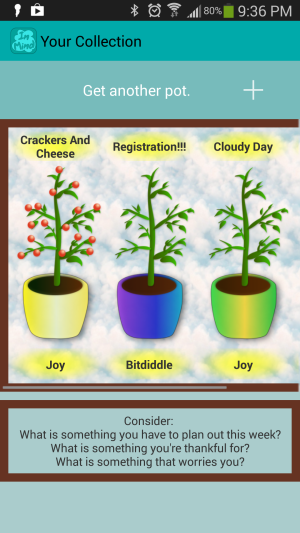
\includegraphics[width=\textwidth]{planter_init.png}
      \caption{Home View v1.0}
    \end{subfigure}
    \begin{subfigure}[b]{0.4\textwidth}
      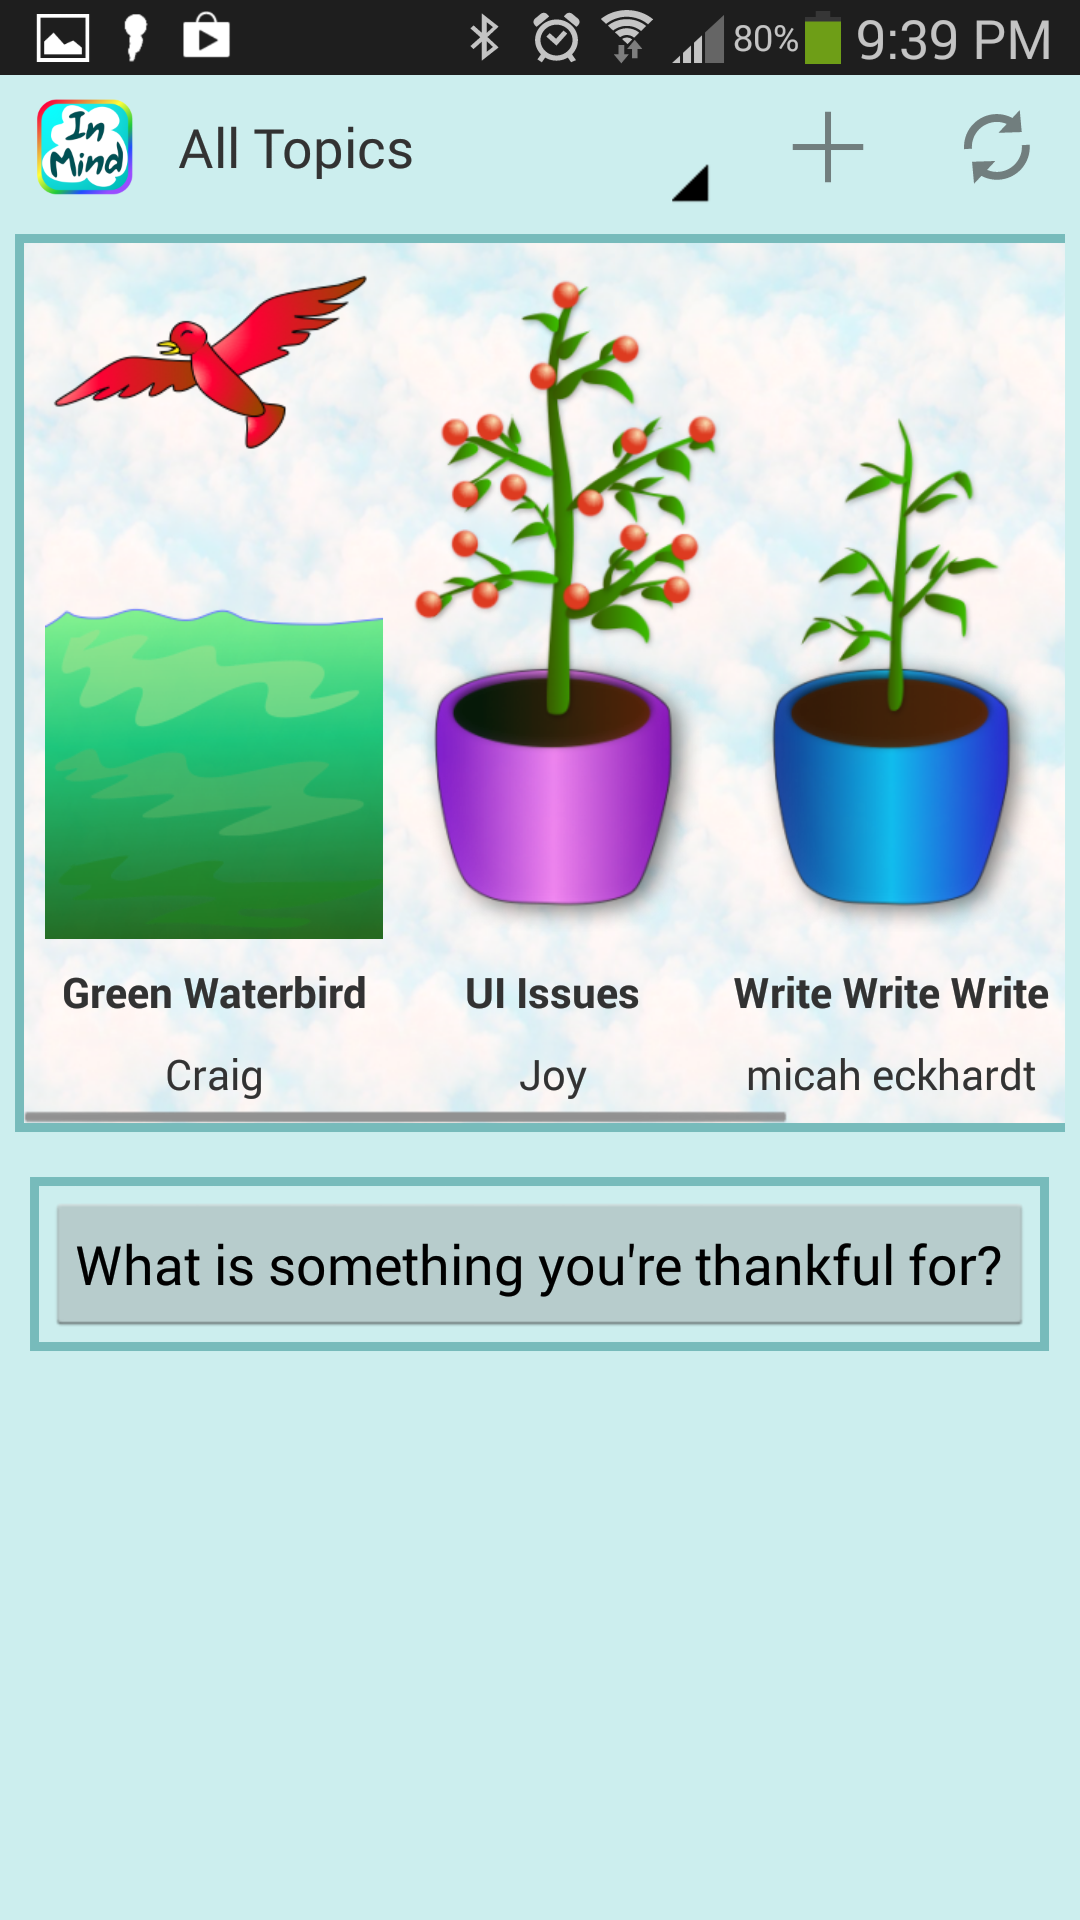
\includegraphics[width=\textwidth]{planter_final.png}
       \caption{Home View v1.4}
    \end{subfigure}
    \label{fig:home_screens}
  \end{figure}

  \begin{figure}
    \caption{\textbf{Evolution of InMind Look and Feel Topic View} --
    On feedback from users, the interface evolved to be more intuitive and attractive.}
    \centering
    \begin{subfigure}[b]{0.4\textwidth}
      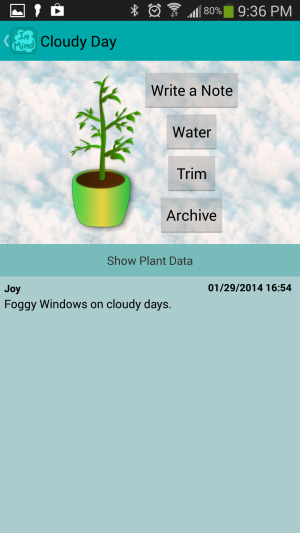
\includegraphics[width=\textwidth]{plant_init.png}
       \caption{Topic View v1.0}
    \end{subfigure}
    \begin{subfigure}[b]{0.4\textwidth}
      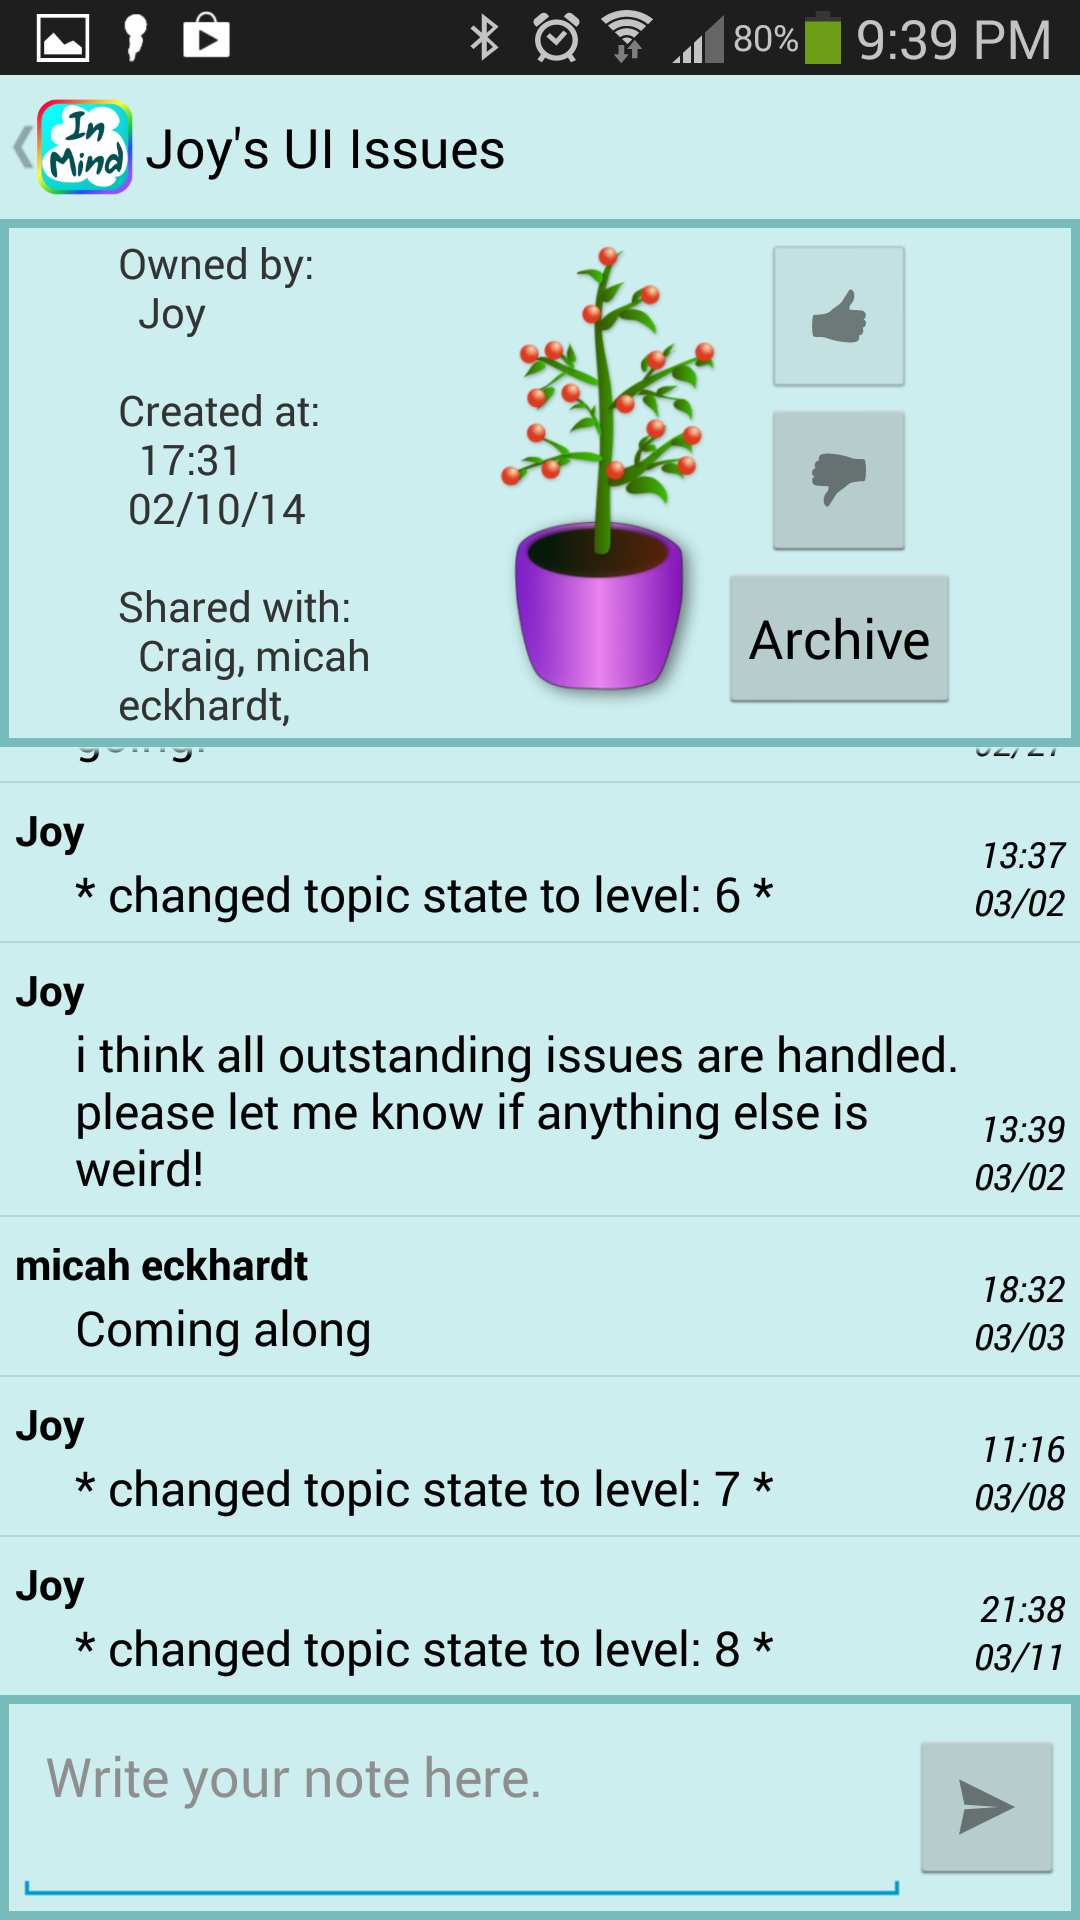
\includegraphics[width=\textwidth]{plant_final.png}
       \caption{Topic View v1.4}
    \end{subfigure}
    \label{fig:topic_screens}
  \end{figure}
